
\section{Implementation}
\label{sec:Implementation}

\subsection{Komponenten}
\label{impl:Komponenten}

\subsection{QGIS Plugin}
\label{impl:QGIS Plugin}
TODO

\subsection{PlazaRoute Container}
\label{impl:PlazaRoute Container}
TODO

\subsubsection{Plaza Vorverarbeitung}
\label{impl:Plaza Vorverarbeitung}
TODO

\subsubsection{Plaza Routing}
\label{impl:Plaza Routing}
TODO

\begin{figure}[ht]
\centering
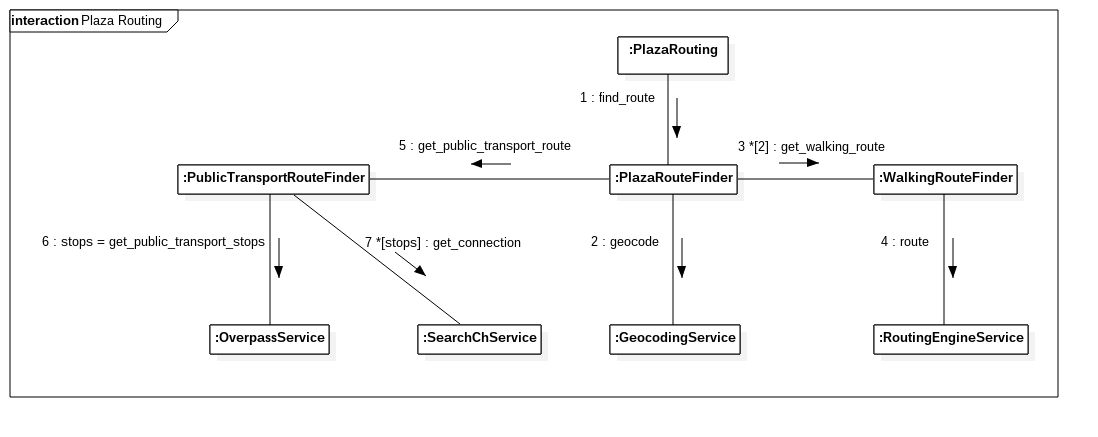
\includegraphics[width=1\linewidth]{projectdoc/img/communication_diagram}
\caption[Plaza Routing Collaboration Diagramm]{Plaza Routing Communication Diagramm}
\label{fig:communication_diagram}
\end{figure}


% Da ÖV-Stationen und -Linien in \ac{OSM} nicht konsistent gemappt sind, wird das Recovery Blocks Pattern \cite{fault_tolerant_software} angewendet, um möglichst ein 
%TODO Problematik mit OSM-Daten und Recovery-Block Pattern in Implementation verschieben
